\title[P\&S 2026/2027]{Probability \& Statistics (Premaster MTPS)}
\subtitle[College 1: introductie in kansrekening]{College 1: introductie in kansrekening}  
\author{Dr. ir. D.A.M.P. Blom}
\institute[NLDA]{Nederlandse Defensie Academie}
\date{25 september 2026}
\begin{document}

\begin{frame}
    \maketitle
    % \begin{center}
    %     \includegraphics[width=3cm]{1_marine}
    %     \includegraphics[width=3cm]{1_luchtmacht}
    %     \includegraphics[width=3cm]{1_landmacht}
    % \end{center}
\end{frame}

%------------------------------------------------%	

\begin{frame}{Even voorstellen}
    \begin{minipage}{0.65\textwidth}
        \begin{itemize}\setlength\itemsep{2em}
            \item Dr. ir. Danny Blom
            \item BSc, MSc, PhD toegepaste wiskunde @ TU Eindhoven
            \item 2024 - heden: universitair docent wiskunde en operations research bij de Faculteit Militaire Wetenschappen (Breda / Den Helder)
            \item Contactinfo:\\ \url{damp.blom@mindef.nl} / forum op Moodle
        \end{itemize}
    \end{minipage}
    \hfill
    \begin{minipage}{0.25\textwidth}
        
\includegraphics[width=\linewidth]{../figures/1_danny_blom.jpg}
    \end{minipage}
\end{frame}

\begin{frame}{Structuur van het vak}
    \begin{itemize}
        \item $20$ \enquote{learning tasks} --- streef naar twee learning tasks per week.
        \item Voornamelijk op zelfstudie, maar ook vier fysieke colleges:
    \end{itemize}
    \vfill
    \begin{center}
        \begin{tabular}{lll}
            \toprule
                \textbf{College 1} & 25 september 2026 & 12.50-16.40 uur \\
                \textbf{College 2} & 16 oktober 2026 & 9.20-16.40 uur \\
                \textbf{College 3} & 6 november 2026 & 9.20-16.40 uur\\
                \textbf{College 4} & 27 november 2026 & 9.20-16.40 uur \\
            \midrule
                \textbf{Tentamen (\SI{100}{\percent})} & 4 december 2026 & n.n.b. \\
                \textbf{Hertentamen} & 12 maart 2026 & n.n.b. \\
            \bottomrule
        \end{tabular}
    \end{center}
    \vfill
    \textbf{Locatie:} raadpleeg het rooster in Eduflex
\end{frame}

\begin{frame}{Cursusdoelen}
    Aan het eind van deze premaster cursus is de student in staat om:
    \begin{enumerate}
        \item verzamelde data met statistische maten te beschrijven.
        \item deze data te verwerken met statistische software (grafische rekenmachine)
        \item te rekenen met (conditionele) kansen.
        \item de principes van discrete / continue kansverdelingen te hanteren.
        \item te rekenen met een aantal veelgebruikte kansverdelingen.
        \item kwantitatieve maten (verwachtingswaarde, variantie, covariantie, regressielijn en de correlatiecoëfficiënt) te berekenen
        \item de centrale limietstelling toe te passen.
        \item te werken met een aantal schattingsmethoden, betrouwbaarheidsintervallen en hypothesetoetsen en benodigde steekproefgroottes te berekenen.
    \end{enumerate}
\end{frame}

\begin{frame}{Leermiddelen}
    \begin{itemize}\setlength\itemsep{2em}
        \item Slides van de vier hoorcolleges 
        \item Boek:
        \begin{itemize}
            \item Douglas Montgomery and George Runger. \emph{Applied Statistics and Probability for Engineers}. 6th International Student Version. ISBN 978-1-118-74412-3
        \end{itemize}
        \item Moodle pagina met lecture notes, opgavensets, antwoorden en uitgebreide uitwerkingen van geselecteerde opgaven.
        \item Grafische rekenmachine: TI84-Plus CE-T of Casio fx-CG50    
    \end{itemize}
    \vfill
    \begin{center}
        \underline{\bfseries Maak gebruik van het forum op Moodle op vragen te stellen!}
    \end{center}
\end{frame}

\begin{frame}{Vandaag}
    \begin{itemize}\setlength\itemsep{2em}
        \item Militaire voorbeelden van kansrekening en onzekerheid
        \item Fundamenten en rekenregels van de kansrekening
        \item Introductie in kansvariabelen
        \begin{itemize}
            \item Kansmassafunctie (PMF)
            \item Cumulatieve verdelingsfunctie (CDF)
            \item Verwachtingswaarde, variantie en standaardafwijking
        \end{itemize}
    \end{itemize}
    \vfill
    \textbf{Dit komt ruwweg overeen met de inhoud van learning tasks 1 t/m 3.}
\end{frame}

\begin{frame}{Kansrekening in de militaire praktijk}
    Een circuit van componenten is functioneel als er een pad bestaat van werkende componenten van links naar rechts:
    \vfill
    \textbf{Deterministisch:} iedere component functioneert met kans $1$.
    Wat is de kans dat het circuit functioneert?
    \vfill
    \begin{center}
        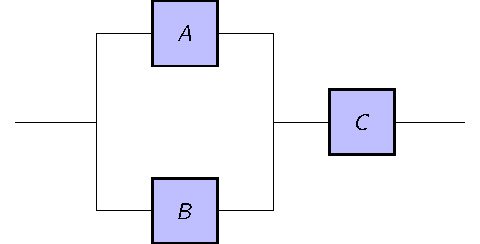
\includegraphics[page=1, width=0.5\textwidth]{../tikz/1_example_circuit.pdf}%
    \end{center}
    \vfill\pause
    \textbf{Flauw voorbeeld: het circuit functioneert met kans $1$ (geen uitval).}
\end{frame}

\begin{frame}{Kansrekening in de militaire praktijk}
    In de praktijk is er echter een hoop onzekerheid over het faalgedrag van componenten.
    \vfill
    \textbf{Stochastisch:} voor iedere component is de kans op functioneren een getal op het interval $[0, 1]$, onafhankelijk van elkaar.
    Wat is de kans dat het circuit functioneert?
    \vfill
    \begin{center}
        \includegraphics[page=2, width=0.5\textwidth]{../tikz/1_example_circuit.pdf}%
    \end{center}
\end{frame}

\begin{frame}{Kansrekening in de militaire praktijk}
    \begin{center}
        \includegraphics[page=2, width=0.5\textwidth]{../tikz/1_example_circuit.pdf}%
    \end{center}
    \vfill
    Dit stochastische geval is al lastiger. 
    We gaan vandaag de nodige tools bekijken om dit op te kunnen lossen!
\end{frame}

\begin{frame}{Kansrekening in de militaire praktijk}
    In de militaire praktijk hebben we heel vaak te maken met onzekerheid.
    \begin{itemize}\setlength\itemsep{1.5em}
        \item Strategie coördineren bij het zoeken naar vijandelijke onderzeeboten.
        \item Betrouwbaarheid van communicatiesystemen analyseren.
        \item Welke reserveonderdelen (\enquote{spare parts}) moeten we meenemen op een missie?
        \item Hoeveel slachtoffers krijgt de medische keten te verwerken bij een \enquote{mass casualty event}?
        \item Welke invloed hebben meteorologische verschijnselen op raketbanen?
    \end{itemize}
\end{frame}

\begin{frame}{Kansexperiment: worp met twee dobbelstenen}
    Wat voor eigenschappen heeft een dergelijk \concept{kansexperiment}?
    
    \only<1>{
       \color{white} De uitkomstenruimte (\emph{sample space}) is als volgt:\medskip
    }
    \only<2>{
        \begin{itemize}
            \item De \concept{uitkomstenruimte} (\emph{sample space}) is als volgt:
        \end{itemize}
    }
    \only<3>{
        \begin{itemize}
            \item De \concept{kansverdeling over de uitkomstenruimte} is als volgt:
        \end{itemize}
    }
    \only<4>{
        \begin{itemize}
            \item \concept{Trekking} van exact één van de uitkomsten in de uitkomstenruimte:
        \end{itemize}
    }
    \begin{center}
        \centering
        \foreach \ov in {1,...,4}{% 
            \only<\ov>{%
                
\includegraphics[page=\ov, width=0.5\textwidth]{../tikz/1_rolling_dice.pdf}%
            }%
        }%
    \end{center}
\end{frame}

\begin{frame}{Kansexperiment}
    \textbf{Input:} \medskip

    \begin{itemize}
        \item Uitkomstenruimte $S$
        \item Onderliggende kansverdeling over $S$
    \end{itemize}\medskip

    \textbf{Experiment:} \medskip

    \begin{itemize}
        \item Lab-meting
        \item Afname van een enquête
        \item Simulatie
        \item $\ldots$
    \end{itemize}\medskip

    \textbf{Output:} \medskip

    \begin{itemize}
        \item Een trekking van exact één van de uitkomsten in de uitkomstenruimte
    \end{itemize}
\end{frame}

\begin{frame}{Gebeurtenissen}
    Vaak zijn er niet geïnteresseerd in de kans op één specifieke uitkomst, maar de kans op een \concept{gebeurtenis} (\emph{event}):

    \begin{itemize}
        \item Gebeurtenis $A$: er wordt minstens één drie gegooid:
        \[
            A = \set{(3,1), (3,2), (3,3), \ldots, (4, 3), (5, 3), (6, 3)}
        \]
        \item Gebeurtenis $B$: de som van de twee worpen is gelijk aan $7$:
        \[
            B = \set{(1,6), (2,5), (3,4), (4,3), (5,2), (6,1)}
        \]
    \end{itemize}
    \vfill
    \textbf{Algemeen:} een gebeurtenis $E$ is een deelverzameling van de uitkomstenruimte (notatie: $E \subseteq S$). 
    De kans $P(E)$ is dan de kans dat één van de uitkomsten in de deelverzameling $E$ wordt gerealiseerd.
\end{frame}

\begin{frame}{Samenstellingen van gebeurtenissen}
    Gebeurtenissen kunnen we ook grafisch weergeven met behulp van \concept{Venndiagrammen}:\medskip

    Hiermee kunnen we ook weer samenstellingen van gebeurtenissen bekijken:
    \vfill
    \begin{center}
        \centering
        \foreach \ov in {1,...,5}{% 
            \only<\ov>{%
                \includegraphics[page=\ov, width=0.75\textwidth]{../tikz/venn_diagrams.pdf}%
            }%
        }%
    \end{center}
\end{frame}

\begin{frame}{Axioma's van de kansrekening}
    Stel nu dat we een kansexperiment hebben met een uitkomstenruimte $S$, en een gebeurtenis $E \subseteq S$.
    \vfill
    Een \concept{kansfunctie} $P$ is een functie die aan iedere gebeurtenis $E$ een getal toekent zodat het volgende geldt:
    \begin{itemize}[<+->]
        \item $P(S) = 1$.
        \item $0 \leq P(E) \leq 1$ voor iedere gebeurtenis $E$.
        \item Als twee gebeurtenissen $E_1$ en $E_2$ een lege doorsnede hebben (notatie: $E_1 \cap E_2 = \emptyset$), dan geldt:
        \[
            P(E_1 \cup E_2) = P(E_1) + P(E_2).
        \]
    \end{itemize}
\end{frame}

\begin{frame}{Handige rekenregels voor kansrekening}
    Met deze axioma's kunnen we een aantal handige rekenregels afleiden:
    \begin{itemize}\setlength\itemsep{3em}
        \item Voor een gebeurtenis $E$ geldt dat de uitkomstenruimte $S$ kan worden opgedeeld in $E$ en haar complement $E'$ ($S = E \cup E'$), oftewel 
        \[
            P(S) = P(E \cup E') = P(E) + P(E') = 1
        \]
        Hieruit volgt:\bigskip
        
        $P(E) = 1 - P(E')$ \hfill (\concept{complementregel})
        
        \item Als we de kansen van twee gebeurtenissen $E_1$ en $E_2$ optellen, dan wordt de doorsnede $E_1 \cap E_2$ dubbel geteld, oftewel:\bigskip
        
        $P(E_1 \cup E_2) = P(E_1) + P(E_2) - P(E_1 \cap E_2)$ \hfill (\concept{algemene optelregel})
    \end{itemize}
\end{frame}

\begin{frame}{Oefening: worp met twee dobbelstenen}
    \begin{itemize}
        \item Gebeurtenis $A$: er wordt minstens één vier gegooid.
        \item Gebeurtenis $B$: de som van de twee worpen is gelijk aan $7$.
        \item Gebeurtenis $C$: het product van de twee worpen is gelijk aan $10$.
    \end{itemize}
    \vfill
    \begin{enumerate}\setlength\itemsep{2em}
        \item Teken de gebeurtenissen $A$, $B$ en $C$ als een Venndiagram.
        \item Wat is de kans dat gebeurtenis $B$ \textbf{niet} plaatsvindt?
        \item Wat is de kans dat minstens één van beide gebeurtenissen $A$ of $B$ plaatsvindt?
        \item Wat is de kans dat zowel $A$ als $C$ plaatsvindt?
    \end{enumerate}
\end{frame}

\begin{frame}{Oefening: worp met twee dobbelstenen}
    \only<+>{
        \textbf{Teken de gebeurtenissen $A$, $B$ en $C$ als een Venndiagram.}\bigskip

        \begin{center}
            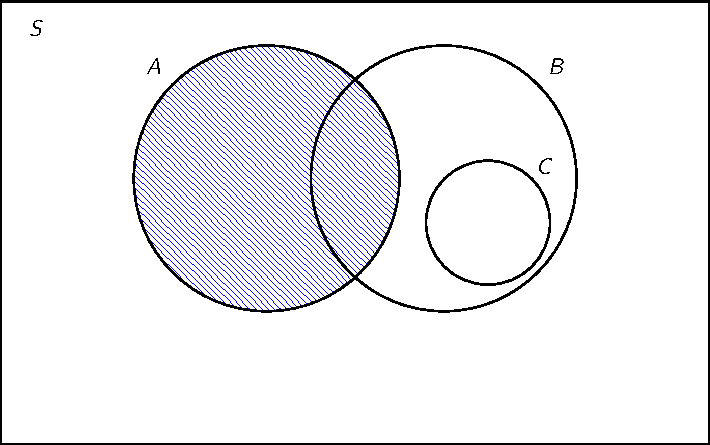
\includegraphics[scale=0.7]{../tikz/1_example_events.pdf}
        \end{center}
    }

    \only<+>{
        \textbf{Wat is de kans dat gebeurtenis $B$ niet plaatsvindt?}\bigskip

        $B$ bestaat uit $6$ uitkomsten, dus $P(B) = \frac{6}{36}$.
        Met de complementregel vinden we dan 
        \begin{align*}
            P(B')  &= 1 - P(B) \\
                        &= 1 - \frac{6}{36} \\
                        &= \frac{30}{36} = \frac{5}{6}.
        \end{align*}
    }

    \only<+>{
        \textbf{Wat is de kans dat minstens één van beide gebeurtenissen $A$ of $B$ plaatsvindt?}\bigskip

        $A$ bestaat uit $11$ uitkomsten, $B$ bestaat uit $6$ uitkomsten, en $A \cap B$ bestaat uit $2$ uitkomsten, oftewel 
        \begin{itemize}
            \item $P(A) = \frac{11}{36}$
            \item $P(B) = \frac{6}{36}$
            \item $P(A \cap B) = \frac{2}{36}$
        \end{itemize}
        Met de algemene optelregel vinden we dan 
        \begin{align*}
            P(A \cup B) &= P(A) + P(B) - P(A \cap B) \\
                        &= \frac{11}{36} + \frac{6}{36} - \frac{2}{36} \\
                        &= \frac{15}{36}.
        \end{align*}
    }

    \only<+>{
        \textbf{Wat is de kans dat zowel $A$ als $C$ plaatsvindt?}\bigskip

        Deze kans is gelijk aan $0$. \vfill
        
        Gebeurtenis $C$ (product gelijk aan $10$) vindt alleen plaats als er een $2$ en een $5$ worden gegooid. \vfill
        
        Dat betekent dat $A$ (minstens één vier gooien) niet kan plaatsvinden, oftewel de gebeurtenissen $A$ en $C$ kunnen niet tegelijkertijd plaatsvinden.
    }
\end{frame}

\begin{frame}{Voorbeeld: performance van een C-UAS systeem}
    Het C-UAS peloton van 11 Luchtverdedigingsbatterij bewaakt een sector rond een tijdelijke operatiebasis.
    Ze gebruiken een radar/RF-detectiesysteem dat automatisch alarm slaat wanneer het een mogelijk vijandelijke drone waarneemt.
    Van alle objecten die door de lucht de basis naderen, blijkt \SI{10}{\percent} een vijandelijke drone te zijn.
    Als er daadwerkelijk een vijandelijke drone is, wordt in \SI{94}{\percent} van de gevallen daadwerkelijk alarm geslagen.
    Als het niet om een vijandelijke drone gaat, wordt in \SI{5}{\percent} van de gevallen alarm geslagen, bijvoorbeeld wanneer het systeem
    niet kan onderscheiden van vogels of onwetende hobbydrones.
    \vfill
    \textbf{Wat is de kans dat het dronesysteem de verkeerde beslissing neemt bij een willekeurig naderend object?}
\end{frame}

\begin{frame}{Voorbeeld: performance van een C-UAS systeem}
    \begin{center}
        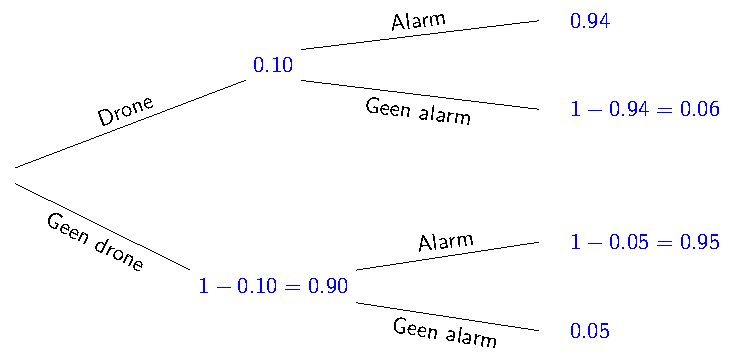
\includegraphics[page=1, width=0.9\textwidth]{../tikz/1_cuas_system.pdf}%
    \end{center}
\end{frame}

\begin{frame}{Voorbeeld: performance van een C-UAS systeem}
    We kunnen dit nu ook opschrijven in termen van gebeurtenissen:
    \begin{itemize}
        \item $A$ is de gebeurtenis dat alarm wordt geslagen.
        \item $D$ is de gebeurtenis dat we met een vijandelijke drone te maken hebben.
    \end{itemize}
    \vfill
    Merk op dat de kansen dat alarm wordt geslagen afhankelijk is van of we echt met een vijandelijke drone te maken hebben.
    We werken hier dus met \concept{voorwaardelijke kansen}:
    \begin{itemize}
        \item Kans op een drone is $P(D) = 0.06$.
        \item Kans op alarm gegeven dat het een drone is: $P(A | D) = 0.94$
        \item Kans op alarm gegeven dat het niet een drone is: $P(A | D') = 0.05$. 
    \end{itemize}
\end{frame}

\begin{frame}{Voorbeeld: performance van een C-UAS systeem}
    Bekijk nu de bovenste tak:
    \begin{center}
        \includegraphics[page=2, width=\textwidth]{../tikz/1_cuas_system.pdf}%
    \end{center}
    In \SI{10}{\percent} van de gevallen gaat het om een vijandelijke drone, en weer \SI{94}{\percent} van de gevallen daarvan wordt alarm geslagen:
    Met andere woorden:
    \[
        P(D \cap A) = P(D) \cdot P(A | D) \Rightarrow P(A | D) = \frac{P(D \cap A)}{P(D)}
    \]
\end{frame}

\begin{frame}{Voorbeeld: performance van een C-UAS systeem}
    \textbf{In hoeveel procent van de gevallen wordt er alarm geslagen?}\pause\vfill
    \begin{center}
        \only<3>{%
            \includegraphics[page=3, width=0.7\textwidth]{../tikz/1_cuas_system.pdf}%
        }%
        \only<4->{%
            \includegraphics[page=4, width=0.7\textwidth]{../tikz/1_cuas_system.pdf}%
        }
    \end{center}
    \begin{center}
        \begin{tabular}{ll}
            \uncover<3->{Alarm en drone:        & $P(A \cap D) = P(D) \cdot P(A | D) = 0.094$ \\}%
            \uncover<4->{Alarm en geen drone:   & $P(A \cap D') = P(D') \cdot P(A | D') = 0.045$ \\}%
        \end{tabular}
    \end{center}
    
    \onslide<5->{
        Totale kans op een alarm is dus:
        \[
            P(A) = P(A \cap D) + P(A \cap D') = 0.094 + 0.045 = 0.139.
        \]
    }
\end{frame}

\begin{frame}{Wet van de totale kans}
    In algemene zin kunnen we de kans op één specifieke gebeurtenis bepalen aan de hand van een aantal voorwaardelijke kansen:
    \vfill
    Als we de uitkomstenruimte kunnen opdelen in gebeurtenissen $B_1, B_2, \ldots, B_n$, dan geldt:
    \vfill
    \begin{align*}
        P(A)    &= P(A \cap B_1) + P(A \cap B_2) + \ldots + P(A \cap B_n) \\
                &= P(B_1) \cdot P(A | B_1) + P(B_2) \cdot P(A | B_2) + \ldots + P(B_n) \cdot P(A | B_n)
    \end{align*}
    \vfill
    \textbf{Merk op: $D$ en $D'$ delen de uitkomstenruimte op in twee!}
\end{frame}

\begin{frame}{Oefening: performance van een C-UAS systeem}
    Het C-UAS peloton van 11 Luchtverdedigingsbatterij bewaakt een sector rond een tijdelijke operatiebasis.
    Ze gebruiken een radar/RF-detectiesysteem dat automatisch alarm slaat wanneer het een mogelijk vijandelijke drone waarneemt.
    Van alle objecten die door de lucht de basis naderen, blijkt \SI{10}{\percent} een vijandelijke drone te zijn.
    Als er daadwerkelijk een vijandelijke drone is, wordt in \SI{94}{\percent} van de gevallen daadwerkelijk alarm geslagen.
    Als het niet om een vijandelijke drone gaat, wordt in \SI{5}{\percent} van de gevallen alarm geslagen, bijvoorbeeld wanneer het systeem
    niet kan onderscheiden van vogels of onwetende hobbydrones.
    \vfill
    \textbf{Wat is de kans dat het dronesysteem de verkeerde beslissing neemt bij een willekeurig naderend object?}
    
\end{frame}

\begin{frame}{Onafhankelijkheid}
    \textbf{Tot nu toe:} kans op een bepaalde gebeurtenis verandert zodra we extra informatie hebben (voorwaardelijke kansen).
    \vfill
    Maar wat als deze extra informatie geen verschil maakt?
    \vfill
    We noemen twee gebeurtenissen $A$ en $B$ \concept{onafhankelijk} als geldt:
    \[
        P(A | B) = P(A)
    \]
    \textbf{Gevolg:} bij onafhankelijke gebeurtenissen $A$ en $B$ mogen we kansen vermenigvuldigen als we de doorsnede $A \cap B$ bekijken:
    \[
        P(A \cap B) = P(B) \cdot P(A | B) = P(B) \cdot P(A)
    \]
\end{frame}

\begin{frame}{Recap: faalgedrag van componenten}
    \begin{center}
        \includegraphics[page=2, width=0.5\textwidth]{../tikz/1_example_circuit.pdf}%
    \end{center}
    \vfill
    Het circuit functioneert wanneer er een pad van links naar rechts is van functionerende componenten.
    Per component is de faalkans weergegeven (kans dat de component niet functioneert) en de faalgedrag van componenten is onafhankelijk.\bigskip

    \textbf{Bereken de kans dat het circuit functioneert.}
\end{frame}

\begin{frame}{Bereken de kans op functioneren van dit circuit}
    We bekijken gebeurtenissen $A, B, C$ dat component $A, B, C$ blijven functioneren.
    Het circuit functioneert als:
    \begin{itemize}
        \item Minstens één van $A$ of $B$ blijft functioneren.
        \item $C$ blijft functioneren.
    \end{itemize}
    We willen dus $P\left((A\cup B) \cap C\right)$ berekenen:

    \begin{align*}
        \uncover<1->{P(A) &= 0.95,\qquad P(B) = 0.88 \qquad \text{ en } P(C) = 0.92. \\[2ex]}
        \uncover<2->{P(A \cup B)     &= P(A) + P(B) - P(A \cap B) \\
                            &= P(A) + P(B) - P(A) \cdot P(B) \\
                            &= 0.95 + 0.88 - 0.95 \cdot 0.88 \\
                            &= 0.994.\\[2ex]}
        \uncover<3->{P((A\cup B) \cap C) &= P(A \cup B) \cdot P(C) = 0.994 \cdot 0.92 = 0.91448}
    \end{align*}
\end{frame}

\begin{frame}{Voorbeeld: performance van een C-UAS systeem}
    Het C-UAS peloton van 11 Luchtverdedigingsbatterij bewaakt een sector rond een tijdelijke operatiebasis.
    Ze gebruiken een radar/RF-detectiesysteem dat automatisch alarm slaat wanneer het een mogelijk vijandelijke drone waarneemt.
    Van alle objecten die door de lucht de basis naderen, blijkt \SI{10}{\percent} een vijandelijke drone te zijn.
    Als er daadwerkelijk een vijandelijke drone is, wordt in \SI{94}{\percent} van de gevallen daadwerkelijk alarm geslagen.
    Als het niet om een vijandelijke drone gaat, wordt in \SI{5}{\percent} van de gevallen alarm geslagen, bijvoorbeeld wanneer het systeem
    niet kan onderscheiden van vogels of onwetende hobbydrones.
    \vfill
    \textbf{Stel nu dat het alarm afgaat. Wat is de kans dat het nu echt gaat om een vijandelijke drone?}
\end{frame}

\begin{frame}{Voorbeeld: performance van een C-UAS systeem}
    \begin{center}
        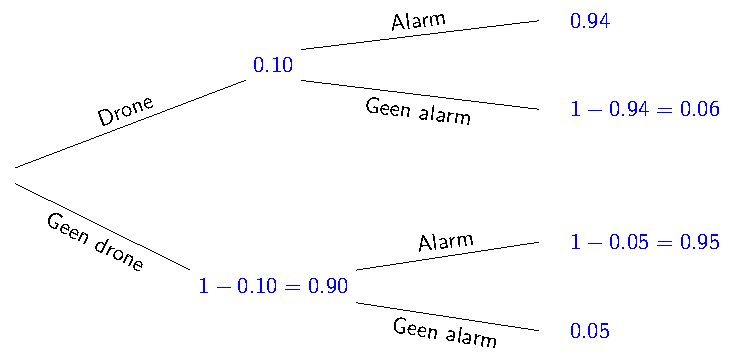
\includegraphics[page=1, width=0.65\textwidth]{../tikz/1_cuas_system.pdf}%
    \end{center}
    Uit het boomdiagram kunnen we een aantal kansen afleiden:
    \begin{itemize}
        \item $P(D) = 0.10$ en $P(D') = 0.90$.
        \item $P(A | D) = 0.94$,  $P(A' | D) = 0.06$, $P(A | D') = 0.05$, $P(A' | D') = 0.95$.
    \end{itemize}
    \vfill
    \textbf{We willen echter de kans $P(D | A)$ berekenen! Hoe kunnen we dat doen?}
\end{frame}

\begin{frame}{Voorbeeld: performance van een C-UAS systeem}
    Merk op dat we de kans $P(A \cap D)$ op twee manieren kunnen schrijven:
    \begin{itemize}
        \item $P(A \cap D) = P(A) \cdot P(D | A)$
        \item $P(A \cap D) = P(D) \cdot P(A | D)$
    \end{itemize}
    Met andere woorden, de rechterkanten moeten hetzelfde zijn:
    \[
        P(A) \cdot P(D | A) = P(D) \cdot P(A | D)
    \]
    
    Eerder hebben we berekend dat $P(A) = 0.139$, en $P(D) = 0.10$ en $P(A | D) = 0.94$:
    \[
        0.139 \cdot P(D | A) = 0.10 \cdot 0.94 \Rightarrow P(D | A) = \frac{0.10 \cdot 0.94}{0.139} = 0.6763.
    \]
\end{frame}

\begin{frame}{Bayes' regel}
    Deze rekenregel, waarbij we voorwaardelijke kans kunnen \enquote{omdraaien}, noemen we ook wel \concept{Bayes' regel}:\vfill

    Voor gebeurtenissen $A$ en $B$ waarbij $P(A) > 0$ geldt dat:
    \[
        P(B | A) = \frac{P(A | B) \cdot P(B)}{P(A)}
    \]
    (de voorwaarde $P(A) > 0$ is nodig, omdat anders gedeeld wordt door $0$).
\end{frame}

\begin{frame}{Kansvariabelen}
    Tot nu toe hebben we vooral gewerkt met kansexperimenten, zoals het werpen van twee dobbelstenen.
    \begin{itemize}
        \item Uitkomstenruimte $S$
        \item Kansverdeling over $S$
        \item Een trekking uit de uitkomstenruimte $S$.
    \end{itemize}
    \vfill\pause
    Bij een worp met twee dobbelstenen krijg je een uitkomst als $(3, 5)$, maar hier kun je niet handig mee rekenen.
    \vfill\pause
    Hiervoor bekijken we een \concept{kansvariabele} of \concept{stochast}, oftewel een variabele $X$ die iedere mogelijke uitkomst \enquote{vertaalt} naar een getal. 
    \vfill\pause
    \textbf{Voorbeeld:} $X$ is de som van het aantal ogen van twee geworpen dobbelstenen. De uitkomst $(3, 5)$ wordt vertaald naar $8$. 
\end{frame}

\begin{frame}{Kansvariabelen}
    Er zijn twee soorten kansvariabelen: \concept{discrete} en \concept{continue kansvariabelen}:
    \vfill
    \begin{center}
        \begin{tabular}{lll}
            \toprule
                \textbf{Discrete kansvariabelen} & \textbf{Continue kansvariabelen} \\
            \midrule
                Losse, afzonderlijke getallen & Interval van getallen \\
                Tellen of categoriseren       & Meten \\
            \bottomrule       
        \end{tabular}
    \end{center}
    \vfill
    \textbf{Vandaag:} focus op \concept{discrete kansvariabelen}
\end{frame}

\begin{frame}{Discrete kansvariabelen}
    Een \concept{discrete kansvariabele} is een kansvariabele met een \emph{eindige} of \emph{aftelbaar oneindige} uitkomstenruimte van numerieke waarden.

    \textbf{Voorbeelden:}
    \begin{itemize}
        \item Aantal succesvolle \enquote{hits} bij $10$ achtereenvolgende schoten op een doel ($0, 1, \ldots, 10$)
        \item Aantal gedetecteerde onontplofte bommen uit de Tweede Wereldoorlog in Nederland in een week ($0, 1, \ldots$)
        \item Aantal pogingen totdat een cyberaanval slaagt ($1, 2, \ldots$)
        \item Wel of niet detecteren van een vijandelijke drone ($0$ (niet) of $1$ (wel))
    \end{itemize}

\end{frame}

\begin{frame}{Discrete kansvariabelen: kansmassafunctie}
    Een \concept{discrete kansvariabele} is een kansvariabele met een \emph{eindige} of \emph{aftelbaar oneindige} uitkomstenruimte van numerieke waarden.
    \vfill
    De kansverdeling van een discrete kansvariabele kunnen we beschrijven met een \concept{kansmassafunctie} (\emph{probability measure function (PMF)}):
    \vfill
    Voor iedere mogelijke uitkomst $x$ van de discrete kansvariabele $X$ is de kansmassafunctie $f$ gedefinieerd als:
    \[
        f(x) = P(X = x)
    \]
\end{frame}

\begin{frame}{Voorbeeld: nachtelijke infiltratie in vijandelijk gebied}
    Een diepe verkenningspeloton infiltreert 's nachts vijandelijk terrein.
    De inlichtingendienst kan niet met zekerheid zeggen hoeveel vijandelijke patrouilles het peloton zal kruisen.
    \vfill
    Op basis van eerdere satellietbeelden en drone-observaties kan de inlichtingendienst de volgende kansmassafunctie opstellen voor het aantal vijandelijke patrouilles $X$ dat het peloton doorkruist:
    \vfill
   {\small
        \begin{center}
            \begin{tabular}{*{11}{c}}
                \toprule
                    $x$     & $0$ & $1$ & $2$ & $3$ & $4$ & $5$ & $6$ & $7$ & $8$ & $9$ \\
                \midrule    
                    $f(x)$  & $0.10$ & $0.09$ & $0.12$ & $0.07$ & $0.15$ & $0.09$ & $0.08$ & $0.07$ & $0.10$ & $0.13$ \\
                \bottomrule
            \end{tabular}
        \end{center}
    }
\end{frame}

\begin{frame}{Kansmassafunctie}
    De eigenschappen van een kansmassafunctie zijn gelijkaardig aan de axioma's voor kansrekening:
    \vfill
    \begin{itemize}
        \item De kans op een bepaalde uitkomst is altijd een getal tussen $0$ en $1$:
        \[
            0 \leq f(x) \leq 1.
        \]
        \item De som van kansen over alle mogelijke uitkomsten $x$ in een uitkomstenruimte is gelijk aan $1$:
        \[
            \sum_{x \in S} f(x) = 1.
        \]
    \end{itemize}
\end{frame}

\begin{frame}{Verwachtingswaarde}
    De \concept{verwachtingswaarde} (\enquote{expected value}) van een discrete kansvariabele $X$ is de waarde die $X$ \enquote{gemiddeld genomen} zal aannemen:
    \[
        E(X) = \sum_{x \in S} x \cdot f(x) = \sum_{x \in S} x \cdot P(X = x)
    \]
    \vfill
    \textbf{Intuitie: } gewogen gemiddelde van alle mogelijke uitkomsten $x$, met als weging per uitkomst $x$ de kans op die uitkomst $P(X=x)$.
\end{frame}

\begin{frame}{Voorbeeld: nachtelijke infiltratie in vijandelijk gebied}
    
    {\small
        \begin{center}
            \begin{tabular}{*{11}{c}}
                \toprule
                    $x$     & $0$ & $1$ & $2$ & $3$ & $4$ & $5$ & $6$ & $7$ & $8$ & $9$ \\
                \midrule    
                    $f(x)$  & $0.10$ & $0.09$ & $0.12$ & $0.07$ & $0.15$ & $0.09$ & $0.08$ & $0.07$ & $0.10$ & $0.13$ \\
                \bottomrule
            \end{tabular}
        \end{center}
    }

    We berekenen de verwachtingswaarde als volgt:
    \begin{align*}
        E(X)    &= \sum_{x \in S} x \cdot f(x) \\
                &= 0 \cdot f(0) + 1 \cdot f(1) + \ldots + 9 \cdot f(9) \\
                &= 0 \cdot 0.10 + 1 \cdot 0.09 + \ldots + 9 \cdot 0.13 \\
                &= 4.53.
    \end{align*}
    \vfill\pause
    \textbf{Merk op:} de verwachtingswaarde hoeft geen geheel getal te zijn, het gaat om een \enquote{gemiddelde uitkomst} wanneer je dit hypothetische experiment heel vaak zou herhalen
\end{frame}

\begin{frame}{Een gemiddelde vertelt niet het hele verhaal $\ldots$}
    \begin{figure}
        
\includegraphics[width=\textwidth]{1_drowning_statistician.png}
        \caption{https://sketchplanations.com/sneaky-averages}
    \end{figure}

    Ook in de militaire context is het belangrijk om niet alleen naar gemiddelden te kijken, maar ook naar \concept{maten van spreiding}.
\end{frame}

\begin{frame}{Variantie}
    De \concept{variantie} (\enquote{variance}) van een discrete kansvariabele $X$ is de \concept{kwadratische afstand} tot de verwachtingswaarde $E(X)$ die $X$ \enquote{gemiddeld genomen} zal aannemen:
    \[
        \Var{X} = \sum_{x \in S} \left(x - E(X)\right)^2 \cdot f(x) = \sum_{x \in S} \left(x - E(X)\right)^2 \cdot P(X = x)
    \]
    \vfill
    \textbf{Intuitie: } gewogen gemiddelde van alle mogelijke kwadratische afstanden $(x - E(X))^2$, met als weging per uitkomst $x$ de kans op die uitkomst $P(X=x)$.
\end{frame}

\begin{frame}{Voorbeeld: nachtelijke infiltratie in vijandelijk gebied}
    
    {\small
        \begin{center}
            \begin{tabular}{*{11}{c}}
                \toprule
                    $x$     & $0$ & $1$ & $2$ & $3$ & $4$ & $5$ & $6$ & $7$ & $8$ & $9$ \\
                \midrule    
                    $f(x)$  & $0.10$ & $0.09$ & $0.12$ & $0.07$ & $0.15$ & $0.09$ & $0.08$ & $0.07$ & $0.10$ & $0.13$ \\
                \bottomrule
            \end{tabular}
        \end{center}
    }
    We berekenen de variantie als volgt:
    \begin{align*}
        \Var{X} &= \sum_{x \in S} \left(x - E(X)\right)^2 \cdot f(x) \\
                &= \left(0 - E(X)\right)^2 \cdot f(0) + \ldots + \left(9 - E(X)\right)^2 \cdot f(9) \\
                &= \left(0 - 4.53\right)^2 \cdot 0.10 + \ldots + \left(9 - 4.53\right)^2 \cdot 0.13 \\
                &\approx 8.5691.
    \end{align*}
    \vfill\pause
    \textbf{Merk op:} de verwachtingswaarde hoeft geen geheel getal te zijn, het gaat om een \enquote{gemiddelde uitkomst} wanneer je dit hypothetische experiment heel vaak zou herhalen
\end{frame}

\begin{frame}{Standaardafwijking}
    Het nadeel van de variantie is dat het vaak moeilijk te interpreteren is om de waarde groot of klein is, en dat de eenheid van de variantie niet hetzelfde is als de eenheid van de variabele.
    \vfill
    Om die reden wordt vaker de \concept{standaardafwijking} $\sigma(X)$ bestudeerd.
    Deze vinden we door de wortel uit de variantie te nemen:
    \[
        \sigma(X) = \sqrt{\Var{X}}.
    \]\pause
    \vfill
    \textbf{Voorbeeld:}
    \[
        \sigma(X)  = \sqrt{\Var{X}} = \sqrt{8.5691} \approx 2.9273.
    \]
\end{frame}

\begin{frame}{Discrete kansvariabelen: cumulatieve verdelingsfunctie}
    Een \concept{discrete kansvariabele} is een kansvariabele met een \emph{eindige} of \emph{aftelbaar oneindige} uitkomstenruimte van numerieke waarden.
    \vfill
    Een alternatieve manier om de kansverdeling van een discrete kansvariabele te beschrijven is door middel van
    de \concept{cumulatieve verdelingsfunctie} (\emph{cumulative distribution function (CDF)}):
    \vfill
    Nu kijken we niet naar de kans op een uitkomst $x$, maar de kans op \emph{hoogstens} een uitkomst $x$:
    \[
        F(x) = P(X \leq x)
    \]
\end{frame}

\begin{frame}{Cumulatieve verdelingsfunctie}
    Een diepe verkenningspeloton infiltreert 's nachts vijandelijk terrein.
    De inlichtingendienst kan niet met zekerheid zeggen hoeveel vijandelijke patrouilles het peloton zal kruisen.
    \vfill
    Op basis van eerdere satellietbeelden en drone-observaties kan de inlichtingendienst de volgende kansmassafunctie opstellen voor het aantal vijandelijke patrouilles $X$ dat het peloton doorkruist:
    \vfill
   {\small
        \begin{center}
            \begin{tabular}{*{11}{c}}
                \toprule
                    $x$     & $0$ & $1$ & $2$ & $3$ & $4$ & $5$ & $6$ & $7$ & $8$ & $9$ \\
                \midrule    
                    $f(x)$  & \cellcolor<1,3,5,7,9,11,13,15,17,19>{highlightcolor}$0.10$ & \cellcolor<3,5,7,9,11,13,15,17,19>{highlightcolor}$0.09$ & \cellcolor<5,7,9,11,13,15,17,19>{highlightcolor}$0.12$ & \cellcolor<7,9,11,13,15,17,19>{highlightcolor}$0.07$ & \cellcolor<9,11,13,15,17,19>{highlightcolor}$0.15$ & \cellcolor<11,13,15,17,19>{highlightcolor}$0.09$ & \cellcolor<13,15,17,19>{highlightcolor}$0.08$ & \cellcolor<15,17,19>{highlightcolor}$0.07$ & \cellcolor<17,19>{highlightcolor}$0.10$ & \cellcolor<19>{highlightcolor}$0.13$ \\
                \midrule
                    $F(x)$  & \uncover<2->{\cellcolor<2>{highlightcolor}$0.10$} & \uncover<4->{\cellcolor<4>{highlightcolor}$0.19$} & \uncover<6->{\cellcolor<6>{highlightcolor}$0.31$} & \uncover<8->{\cellcolor<8>{highlightcolor}$0.38$} & \uncover<10->{\cellcolor<10>{highlightcolor}$0.53$} & \uncover<12->{\cellcolor<12>{highlightcolor}$0.62$} & \uncover<14->{\cellcolor<14>{highlightcolor}$0.70$} & \uncover<16->{\cellcolor<16>{highlightcolor}$0.77$} & \uncover<18->{\cellcolor<18>{highlightcolor}$0.87$} & \uncover<20->{\cellcolor<20>{highlightcolor}$1$} \\
                \bottomrule
            \end{tabular}
        \end{center}
    }
\end{frame}

\begin{frame}{Cumulatieve verdelingsfunctie}
    
   {\small
        \begin{center}
            \begin{tabular}{*{11}{c}}
                \toprule
                    $x$     & $0$ & $1$ & $2$ & $3$ & $4$ & $5$ & $6$ & $7$ & $8$ & $9$ \\
                \midrule
                    $F(x)$  & $0.10$ & $0.19$ & $0.31$ & $0.38$ & $0.53$ & $0.62$ & $0.70$ & $0.77$ & $0.87$ & $1$ \\
                \bottomrule
            \end{tabular}
        \end{center}
    }
    \vfill
    \begin{enumerate}
        \item Wat is de kans dat er minimaal vijf patrouilles zijn?
        \item Wat is de kans dat er minimaal twee en maximaal zes patrouilles zijn?
    \end{enumerate}
\end{frame}

\begin{frame}{Cumulatieve verdelingsfunctie}
    \textbf{Wat is de kans dat er minimaal vijf patrouilles zijn?}
    {\small
        \begin{center}
            \begin{tabular}{*{11}{c}}
                \toprule
                    $x$     & $0$ & $1$ & $2$ & $3$ & $4$ & $5$ & $6$ & $7$ & $8$ & $9$ \\
                \midrule
                    $F(x)$  & $0.10$ & $0.19$ & $0.31$ & $0.38$ & $0.53$ & $0.62$ & $0.70$ & $0.77$ & $0.87$ & $1$ \\
                \bottomrule
            \end{tabular}
        \end{center}
    }
    \vfill
    De kans die we willen berekenen is dan $P(X \geq 5)$.
    \vfill\pause
    Stel $A$ is de gebeurtenis \enquote{($X \ge 5$)}, dan is het complement $A'$ de gebeurtenis \enquote{($X < 5$)}, oftewel \enquote{($X \leq 4$)}.
    \vfill\pause
    Met de complementregel vinden we dan:
    \[
        P(X \geq 5) = 1 - P(X \leq 4) = 1 - F(4) = 1 - 0.53 = 0.47.
    \]
\end{frame}

\begin{frame}{Cumulatieve verdelingsfunctie}
    \textbf{Wat is de kans dat er minimaal twee en maximaal zes patrouilles zijn?}
    {\small
        \begin{center}
            \begin{tabular}{*{11}{c}}
                \toprule
                    $x$     & $0$ & $1$ & $2$ & $3$ & $4$ & $5$ & $6$ & $7$ & $8$ & $9$ \\
                \midrule
                    $F(x)$  & $0.10$ & $0.19$ & $0.31$ & $0.38$ & $0.53$ & $0.62$ & $0.70$ & $0.77$ & $0.87$ & $1$ \\
                \bottomrule
            \end{tabular}
        \end{center}
    }
    \vfill
    Stel $A$ is de gebeurtenis \enquote{$(X \leq 6)$}, dan is deze op te delen in gebeurtenissen \enquote{$(X \leq 1)$} ($B$) en \enquote{$(2 \leq X \leq 6)$} ($C$).
    \vfill\pause
    Omdat $B$ en $C$ een lege doorsnede hebben, geldt:
    \[
        P(X \leq 6) = P(X \leq 1) + P(2 \leq X \leq 6).
    \]
    \vfill\pause
    Omschrijven geeft:
    \[
        P(2 \leq X \leq 6) = P(X \leq 6) - P(X \leq 1) = F(6) - F(1) = 0.70 - 0.19 = 0.51.
    \]
\end{frame}

\begin{frame}{Samenvatting en vooruitblik}
    \textbf{Volgend college:}
    \begin{itemize}
        \item Fundamenten en rekenregels van de kansrekening
        \item Van kansexperimenten naar kansvariabelen
    \end{itemize}
    \vfill
    \textbf{Volgend college:}
    \begin{itemize}
        \item Continue kansvariabelen
        \item Normale verdeling en de centrale limietstelling
        \item Introductie in de statistiek
    \end{itemize}
\end{frame}

\end{document}